\chapter{Bound Dirichlet Belief Model}\label{ccl}

\section{Introduction}
In this work, we propse Bound Dirichlet Belief Network to address the issue of DirBN model and enlarge the modelling capability. By inserting auxiliary Poisson random variables into the  layerwise connections and appropraite design. This model assumes that there are $N$ objects to be modelled in this word,where $\pi_{i'}$ is used to denote the $i'$-th latent distribution in the $l$-th layer.There are $L$ hidden layers in the deep architure.


\begin{figure}
% \centering % 图片居中
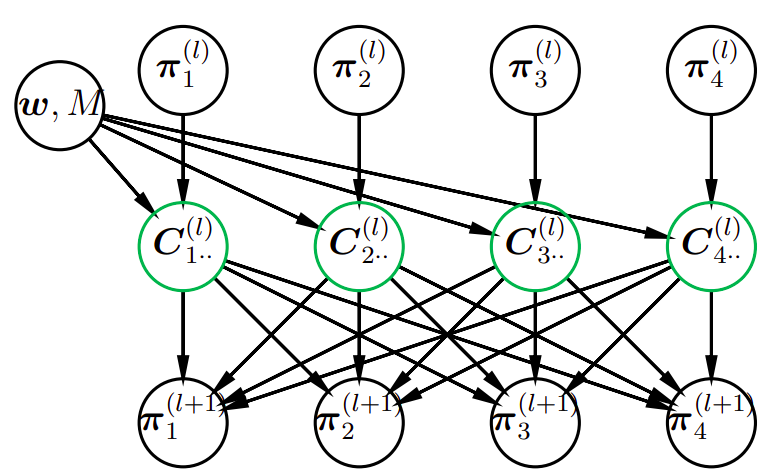
\includegraphics[width = \linewidth]{ubdn.png}
\caption{UBDN Model}
\label{fig:DirBN Model}
\end{figure}

$$ \pi_{i'.}^1 \sim Dirichlet(\beta) $$
$$C_{i'..}^{1} \sim Multi(M^l;\pi_{i'.}^1 \otimes w_{i'.}^l) \tag{1}$$
$$\pi_{i}^{2} \sim Dirihlet(\alpha_d +\sum_{i'}{C_{i'.i}})\tag{2}$$
$$\dots$$
$$C_{i'..}^{l} \sim Multi(M^l;\pi_{i'.}^l \otimes w_{i'.}^l) \tag{1}$$
$$\pi_{i}^{l+1} \sim Dirihlet(\alpha_d +\sum_{i'}{C_{i'.i}^l})\tag{2}$$
\begin{itemize}
  \item Information pass from topic i' to topic i;
  \item $\pi_{i'.}^l$ is the topic-word matrix in layer $l$;
  \item All layer has same number of topic;
  \item $w_{i'i}^l$ is the probability that information pass from topic i' to i;
  \item This process include a reconstruction process;
  \item  $\sum_{i'}{C_{i'.i}}$  is a (V*K) by 1 Vector;
\end{itemize}

where:
$$
M^{(l)} \sim Pisson(M)
$$
\[
w_{i'.}^l \sim Dirichlet(\eta)
\]
Since $\sum_k w_{i'k}^l =1$ ,we can further get :
$$
\sum_{i'}{C_{i'.i}} \sim Multinomial(M^{l};\pi_{i'}^l)
$$
That is to say, the normalized proportion vector can be regard as an approximator of $\pi_{i'}^l$. We reorganiza the counting variables and calculate the recevied counts information for rach node $i$. For any node $i$, it will receive latent counts from all the nodes in this layer. These received counts can then be used to consistute the concentration parameter vector of the receiving node $i's$ Dirichlet distribution.

The number $M^{l}$ of events records the total intensity of relating the latent representation to the related counts. Larger
values of $M^{l}$ will remind a closer approximation to $\pi^{l}$. Further, the introduction of Poisson counts help to decompose the additive effect of the weights, which is quite difficult to have closed Gibbs sampling format.

This key contribution needs to be emphasized again. The
introduction of the counts variable $C$ enables us to use a
layerwise sampling method for all the variables and thus
avoid the complicated strategy of backward counts propagation and forward variable sampling. $C_{i'}^{{l}}$ plays the role of "likelihood" variable for each latent distribution π and we can thus easily obtain Gibbs sampling for $\pi_{i'}^{(l)}$.
 Based on Poisson-Multinomial Equivalence,we can get:
 $$C_{i'ki}^{l} \sim Poisson(M^l \pi_{i'k}^l w_{i'i}^l)\tag{3}$$
 Combining its likelihood, we can easily obtain all its potential posterior proportional
 values.


\section{Inference Process}
Unlike DirBN model which inference latent vairiables by propagating count matrix with Chinese Restaurant Table (CRT) distribution.In DBN model,we can directly use Gibbs sampling stratrgy for model inference. Obivously Dirichlet distribution and multinomial is conjugate so that the posterior dsitribution is alse Dirichlet distribution. The detail of inference is as follow:
\begin{enumerate}
  \item The input matrix of model is a topic-word matrix  $z$ which is a K by V matrix and then sample $\pi_{i'}^{L}$:

  $$\pi_{i'}^{L} \sim Dirichlet(z + C_{i'.i}^L)$$

  \item Sampl $C_{i'ki}^l$.
  $$P(C_{i'ki}^{l}|.) \sim \frac{(M^l \pi_{i'k}^l w_{i'i}^l)^{C_{i'ki}}}{C_{i'ki}^{l}!}$$

  $$P(\pi_i^{l+1}|C_{i'ki}^{l},..) = \frac{1}{B({\alpha_d +\sum_{i'}{C_{i'.i})}}} \prod^V \pi_{ik}^{\alpha_d+C_{i'ki}^l-1}$$

  the posterior distribution of $C_{i'ki}^{l}$ is:

  $$P(C_{i'ki}^{l}|.) \propto \frac{(M^l \pi_{i'k}^l w_{i'i}^l)^{C_{i'ki}}}{C_{i'ki}!} .\frac{1}{B({\alpha_d +\sum_{i'}{C_{i'.i}^{l})}}} \prod^V \pi_{ik}^{\alpha_d+C_{i'ki}^l-1} $$

  given that:

  $$\sum_{k,i}{C_{i'ki}^l} = M^l$$

  then

 $$
    {C_{i'ki}^l} \sim Mult(M^{l} | \frac{C_{i'..}^{l}}{\sum_{k,i} C_{i'ki}^{l}})
 $$


  \item Sample $\pi_{i'}^l$, its posterior distribution is Dirichlet distribution.
  \[
    \pi_{i'..}^l \sim Dirihlet(\alpha_d +\sum_{i'}{C_{i'.i}^{(l-1)}})
  \]
  $$ \pi_{i'.}^1 \sim Dirichlet(\beta) $$
  \[
    \sum_i w_{i'i} = 1
  \]

  then :
    $$\sum_i{C_{i'ki}} \sim Multi(M^l;d\pi_{i'.}^l)$$
    $$
     \pi_{i'.}^l \sim Dirichlet(\eta + \sum_{i'} C_{i'.i}^{l-1} + \sum_i{C_{i'ki}^l})
    $$
    $$
     \pi_{i'.}^1 \sim Dirichlet(\beta +  \sum_i{C_{i'ki}})
    $$

  \item  Sample $w_{i'}$.

  \[
    w_{i'}^l \sim Dirichlet(\eta)
  \]
  Likelihood function:
  $$\sum_k{C_{i'ki}} \sim Multi(M^l;w_{i'.}^l)$$

  Prior distribution:

  $$W_{i'i} \sim Dirichlet(\alpha_w)$$

  Posterior distribution:

  $$p(w_{i'}|..) \sim Dirichlet(\alpha_w+w_{i'.})$$
\end{enumerate}

\section {Experiment}

The experiment was conducted on a real-word datsets called Tag My News (TMN) \cite{data} which contains 32597 RSS news labelled with 7 categories and there are 13370 unique words in the documents.

For UBD model,we set $M = 200,\eta = \beta = 1$. We use 50 \% of data as our training data and make another other half of data as test data.

Firstly, we need to initilize the model from top to down. For example,for the first layer,the $\pi_{i'}^1$ is subject to Dirichlet distribution with the parameter $\beta$ and $\w_{i'.}^1$ also wil be extracted from the dichlet distribution and then sampling other variables layer by layer.

In the experiment, we will test the performance of UDB model with one and UDB model with two layer structure seperately. Finally,
we use perplexity as the evaluation criterion of the model. Obviously as the number of training increases, the value of perplexity continues to decrease.

\begin{figure}[b]
% \centering % 图片居中
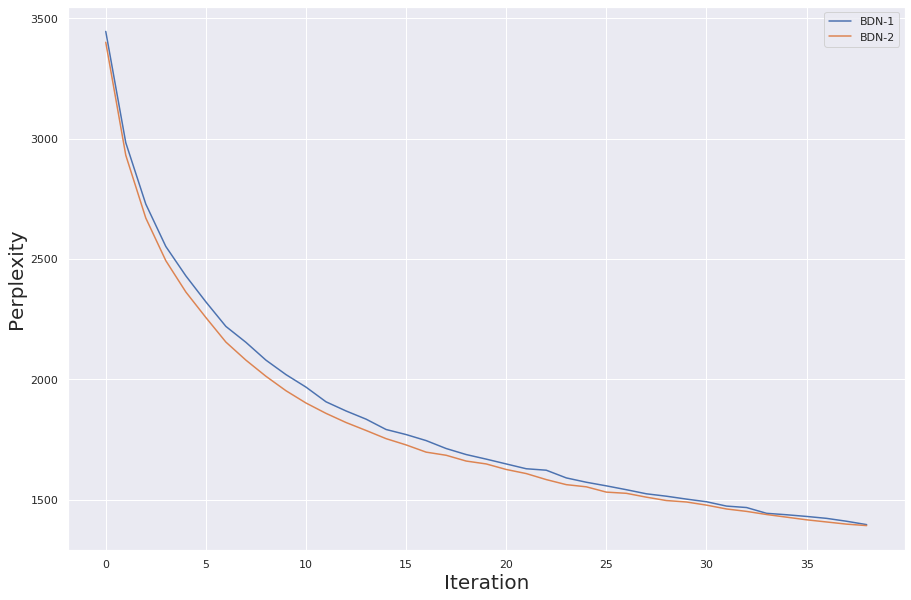
\includegraphics[width = \linewidth]{res.png}
\caption{Result of experiment}
\label{fig:DirBN Model}
\end{figure}


\chapter{Conclusion}\label{ccl}
In this paper, we first introduce the background of Latent Dirichlet Allocation such as bayesian theorem,basic distriubution and the method used in inference process including Gibbs sampling and Metropoli-Hasting sampling.Then we review the generative process of document,inferencing the latent variables in LDA models by Gibbs sampling.

For improving the performance of LDA model,Scientists have done a lot of research on word distribution and topic distribution. However,compared with lots of research on topic structure, word distribution attracts less interest. Zhao\cite{Zhao} proposed Dirichlet belief model to replace dirichlet prior distribution on word distribution,but it is hard for inference latent parameters with complex structure.

We have present a new layerwise inference of Dirichlet Belief Model. With each topic in different layers, DBN model is able to deepen the understanding on topic hierarchies. By inserting auxiliary poisson random variable into the layerwise connections and appropriate design,direct efficient Gibbs sampling over random variables is available.

However,the limitation of this model is that the lengths of latent distrubutions in all the layers are restricted to be the same and need to be fixed.Further directions include introduction of Chinese Restaurant Process on the prior of the length of latent distribution.
